\documentclass[12pt]{article}
 
\usepackage[utf8]{inputenc}
\usepackage[T1]{fontenc}
\usepackage[francais]{babel}
\usepackage{enumerate}
\usepackage{listings}
\usepackage{xcolor}
\usepackage{graphicx}
\usepackage{amssymb}
\usepackage{amsmath}
\usepackage{geometry}
\usepackage{float}
\usepackage{tikz}

\geometry {
	left = 2.5cm,
	right = 2.5cm,
	bottom = 2.5cm ,
	top = 2.5cm ,
}

\lstdefinestyle{customjava}{
 belowcaptionskip=1\baselineskip,
 breaklines=true,
 frame=single,
 %linewidth=7.5cm,
 framexleftmargin=5mm,
 %frameround=tttt,
 %framexrightmargin=5mm,
 xleftmargin=\parindent,
 language=C++,
 showstringspaces=false,
 basicstyle=\footnotesize\ttfamily,
 keywordstyle=\color{green!40!black},
 ndkeywordstyle=\color{orange},
 commentstyle=\color{purple!40!black},
 identifierstyle=\color{blue},
 stringstyle=\color{red},
 numbers=left,
 numbersep=7pt,
}
%06/06/14
\frenchbsetup{StandardLists=true}
\title {Rapport : Format de Fichiers}
\author {Benjamin \emph{VANTHONG}}

\lstset{style=customjava, emph={int,double,void, Double}, emphstyle=\color{red}, emph={[2]wavJava, Spectrum}, emphstyle=[2]\color{orange}}
\begin{document}
\maketitle 
\section {Format de Fichier HDF5}

Durant cette semaine j'ai enfin fini de lire la documentation sur les entrées/sorties HDF5. Afin de tester mes nouvelles connaissances j'ai implémenté un bout de code qui permet d'exporter un fichier au format HDF5 contenant des groupes et des tableaux de données.
\begin{lstlisting}
#include <iostream>
#include <string>

#include "hdf5.h"
#define FILE "test.h5"

int main (void)
{
    const std::string DATASET_NAME ("dset") ;
    std::cout << "HDF5 I/O TEST" << std::endl ;

    hid_t       file_id;   /* file identifier */
    herr_t      status;

    int data [4][6] ;

    for (int i = 0 ; i < 4 ; i ++)
        for (int j = 0 ; j < 6 ; j ++)
            data[i][j] = i * 6 + j ;

    int data1 [4][6] ;

    for (int i = 0 ; i < 4 ; i ++)
        for (int j = 0 ; j < 6 ; j ++)
            data1[i][j] = i * 6 + j + 24 ;

    /* Create a new file */
    file_id = H5Fcreate(FILE, H5F_ACC_TRUNC, H5P_DEFAULT, H5P_DEFAULT);

    hsize_t dims [2] ;
    dims[0] = 4 ;
    dims[1] = 6 ;

    /* Create a dataspace */
    hid_t dataspace_id = H5Screate_simple (2, dims, dims) ;

   
    hid_t group_id = H5Gcreate (file_id, "/Geometry", H5P_DEFAULT, H5P_DEFAULT, H5P_DEFAULT) ;
    hid_t group_id1 = H5Gcreate (file_id, "/Data", H5P_DEFAULT, H5P_DEFAULT, H5P_DEFAULT) ;
    
    /*Create a dataset */
    hid_t dataset_id = H5Dcreate (group_id, "./Nodes", H5T_STD_I32BE, dataspace_id, H5P_DEFAULT, H5P_DEFAULT, H5P_DEFAULT) ;
    hid_t dataset1_id = H5Dcreate (group_id, "./Elements", H5T_STD_I32BE, dataspace_id, H5P_DEFAULT, H5P_DEFAULT, H5P_DEFAULT) ; 
    hid_t dataset2_id = H5Dcreate (group_id1, "./Nodes", H5T_STD_I32BE, dataspace_id, H5P_DEFAULT, H5P_DEFAULT, H5P_DEFAULT) ; 
    hid_t dataset3_id = H5Dcreate (group_id1, "./Elements", H5T_STD_I32BE, dataspace_id, H5P_DEFAULT, H5P_DEFAULT, H5P_DEFAULT) ; 

    H5Dwrite (dataset_id, H5T_NATIVE_INT, H5S_ALL, H5S_ALL, H5P_DEFAULT, data) ;
    H5Dwrite (dataset1_id, H5T_NATIVE_INT, H5S_ALL, H5S_ALL, H5P_DEFAULT, data1) ;
    /* Close dataspace properly */
    status = H5Sclose (dataspace_id) ;
    /* Close dataset properly */
    status = H5Dclose (dataset_id) ;
    status = H5Dclose (dataset1_id) ;
    status = H5Dclose (dataset2_id) ;
    status = H5Dclose (dataset3_id) ;
    /* Close group properly */
    status = H5Gclose (group_id) ;
    status = H5Gclose (group_id1) ;
    /* Terminate access to the file. */
    status = H5Fclose(file_id); 
    return 0;  // successfully terminated

}
\end{lstlisting}
\begin{enumerate}
    \item \textbf{H5Screate\_simple} : créer un dataspace et renvoie son identifiant
    \item \textbf{H5Dcreate} : crée un dataset vide et renvoie son identifiant
    \item \textbf{H5Acreate} : crée un attribut et renvoie son identifiant
    \item \textbf{H5Gcreate} : crée un groupe et renvoie son identfiant
    \item \textbf{H5Dwrite}  : écrit dans un dataset 
\end{enumerate}
\newpage
On peut visualiser le contenu du fichier \emph{test.h5} à l'aide de la commande \emph{h5dump} :\newline
\begin{figure}[h!]
    \begin{center}
        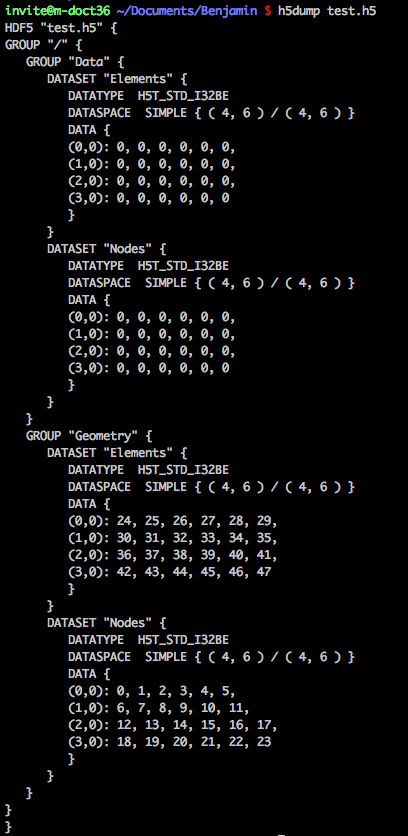
\includegraphics[width=200pt]{test.png}
    \end{center}
\end{figure}
\textbf{Remarque :} J'utiliserai bien sûr la structure du maillage à stocker sous format hdf5 décrite dans le fichier \emph{partitionio.hpp} 
\section {HDF5/XDMF}
Un fichier au format hdf5 ne contient que des données brutes structurées par groupe. Il est donc neccessaire d'utiliser au autre fichier sous format XDMF pour décrire la structure de ses données afin qu'un outil comme paraview puisse interpréter ces données correctement. De ce fait j'ai dû me documenter sur les langages de programmations suivants : HTML, XML, et XDMF.
\section {Travaux à éffectuer}
\begin {enumerate}
    \item - tester les classes dans le fichier "partitionio.hpp" en décommentant des bouts de code.
    \item - étudier la structure du maillage à stocker
    \item - ajouter l'exportation xdmf
\end {enumerate}
\end{document}
